%Style and packages:
%%%%%%%%%%%%%%%%%%%%
\documentclass[prl,superscriptaddress,showpacs,nobalancelastpage,nofootinbib]{revtex4}
%\usepackage{times}
\usepackage{graphicx,amsmath,amsbsy,amssymb}
\usepackage{color}


%New Commands:
%%%%%%%%%%%%%%
\def\one{{\mathchoice {\rm 1\mskip-4mu l} {\rm 1\mskip-4mu l} {\rm
1\mskip-4.5mu l} {\rm 1\mskip-5mu l}}}
\newcommand{\ket}[1]{|{#1}\rangle} \newcommand{\bra}[1]{\langle{#1}|}
\newcommand{\kets}[2]{|{#1}\rangle_{{}_{\!\!{#2}}}}
\newcommand{\bras}[2]{{}_{{}_{{#2}\!\!}}\langle{#1}|}
%\newcommand{\slb}[2]{{{#1}^{({#2})}}} \newcommand{\trace}{\mbox{tr}}
%\renewcommand{\tensor}{\otimes} \newcommand{\vspan}{\mbox{span}}
%\newcommand{\mod}{\mbox{mod}} \newcommand{\lowertr}{\mbox{lt}}
%\newcommand{\diag}{\mbox{dg}} \newcommand{\id}{I}
\newcommand{\comment}[1]{\begin{scriptsize}{\textcolor{green}{[comment:
#1]}}\end{scriptsize}} 
\newcommand{\oldver}[1]{\begin{scriptsize}
{\textcolor{blue}{[Old ver: #1]}}\end {scriptsize}}
\newcommand{\newver}[1]{\textcolor{red}{#1}}


\begin{document}
  
\begin{figure}[htbp]
 \rotatebox{270}{\includegraphics[width=8.5cm,height=12cm]{epfig1.eps}}
 \caption{ The labeled histidine molecule has 14 spin-1/2 nuclei: five
    $^{1}H$, six $^{13}C$ and three $^{15}N$. $H_4$ and $H_5$ are
    indistinguishable (Same chemical shifts and same couplings to the
    other nuclei). Therefore only one qutrit can be encoded into the
    two nuclei. The diagonal of the table shows the chemical shifts of
    each nucleus while the lower triangular terms are the scalar
    couplings values expressed in Hertz. Note that the chemical shifts
    are given with respect to reference frequencies different for each
    nuclear species. The yellow and red spheres represent respectively
    deuterons and oxygen atoms that can be ignored as they do not
    interact with the other spins-1/2. In summary this molecule is a
    register with 12-qubits plus one qutrit. Nevertheless, working
    with the nitrogen nuclei, which are very weakly coupled to the
    other nuclei and have short $T_2s$, leads to long two-qubit gates
    and therefore a large amount of decoherence.  We performed two
    types of transverse relaxation time measurements for each
    spin. First a simple line broadening Lorenzian fit gives us a raw
    estimation on how the spins relax including the static field
    inhomogeneities ($T_2^*$). For the $H_{4/5}$ protons we could not
    get an accurate value because of the broadening of the line
    introduced by the fact that the two protons are not perfectly
    equivalent.  We also performed a serie of spin echo experiments
    to refocus these inhomogeneities and give an close estimate of the
    $T_2$. The values shown in the table corresponds to the sample
    used for the simplified pulse sequence design.}
 \label{Ham_table}
 \end{figure}

\end{document}
